\section{Label-Free Self-Play and How We Measure Ill-Posedness}
\label{sec:setting}

\begin{figure*}[t]
\centering
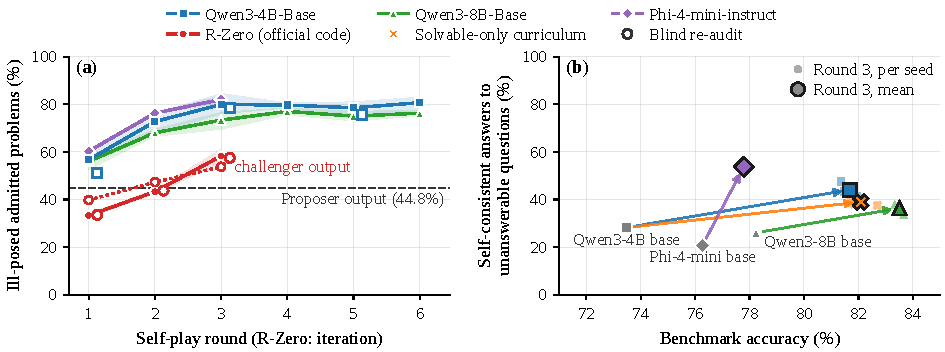
\includegraphics[width=0.88\textwidth]{figures/fig1_drift_harm.pdf}
\caption{(a)~Ill-posed share of admitted problems by round (R-Zero: iteration; mean over seeds, shaded: range). Hollow markers: blind re-judging (Table~\ref{tab:drift}); dashed: all 1,158 first-round proposals of Qwen3-4B-Base, before filtering; dotted: R-Zero's raw challenger output, judged blind. (b)~Self-consistent answers to 600 unanswerable UMWP questions against benchmark accuracy; arrows from each base model to the mean of its round-3 solvers (orange: Qwen3-4B without the ill-posed problems).}
\label{fig:teaser}
\end{figure*}

\paragraph{The loop.} We study the recipe shared by R-Zero and its relatives \citep{huang2026rzero,fang2025serl,chen2025sqlm}: an agreement band decides which problems to train on, and the solver is rewarded for matching its own majority answer, the reward of TTRL \citep{zuo2025ttrl}. In each round, a frozen proposer (the base model) writes 1,200 grade-school math word problems from 40 topic prompts; the current solver samples $G{=}8$ answers to each at temperature 1, and a problem's \emph{agreement} $p$ is the share of samples that give the most frequent answer. The \emph{admission band} keeps a problem when $0.25 \le p \le 0.75$, that is, when two to six of the eight samples agree. This is R-Zero's rule $|p - \frac{1}{2}| \le 0.25$, applied in its paper to ten samples; its code keeps $0.3 \le p \le 0.8$ on nine, the filter our replication runs (both: three to seven agree). The solver then trains for 60 steps on the admitted problems: a rollout earns reward 1 if its answer matches the majority answer of its group of eight, and the advantage is the reward minus the group mean \citep{shao2024deepseekmath}. The round-$t$ curriculum is admitted by the round-$(t{-}1)$ solver (round 1 by the base model); a \emph{lineage} is one seed's sequence of rounds. Each round's candidate pool also contains 200 premise-deleted GSM-Symbolic problems and their 200 intact originals \citep{mirzadeh2025gsmsymbolic}, \emph{planted} to monitor the band. Admitted planted problems are trained on like any other (premise-deleted ones make up 12--23\% of each training set), but all ill-posed shares below refer to proposer-written problems (details: Appendix~\ref{app:setup}).

\paragraph{Models.} We run the loop on Qwen3-4B-Base (five seeds; three continued to round six), Qwen3-8B-Base (three; two to round six), Phi-4-mini-instruct (two), Llama-3.2-3B-Instruct (five) and one round of Qwen3-14B-Base \citep{yang2025qwen3,abouelenin2025phi4mini,grattafiori2024llama3}, and the official R-Zero code on Qwen3-4B-Base.

\paragraph{Measuring ill-posedness.} Claude Opus judges label a random sample of 200 admitted proposer problems per round, under a fixed prompt, as \textsc{solvable} (the text determines a unique numeric answer), \textsc{unsolvable} (a needed quantity or relation is missing, or the conditions contradict each other) or \textsc{ambiguous} (two reasonable readings give different answers), with the rule that a default assumption the reader would have to invent makes a problem unsolvable. A problem is \emph{ill-posed} if it is unsolvable or ambiguous. On 400 questions from UMWP \citep{sun2024umwp} whose answerability was labelled by humans, the judge labels 98.5\% of the unanswerable questions ill-posed and 4.5\% of the answerable ones ($\kappa{=}0.94$; Appendix~\ref{app:judge}). Except where humans labelled them (\S\ref{sec:drift}), ill-posed shares are judge-based estimates. Unless stated otherwise, 95\% intervals resample problems within each seed and round, so they omit variation between seeds, which per-seed ranges show; contrasts between trained models use seed-level $t$-intervals.

\paragraph{Measuring behaviour on unanswerable questions.} Our primary probe is UMWP: 600 unanswerable questions and their 600 answerable originals, with eight samples per question. A model \emph{answers self-consistently} when its most frequent numeric answer holds at least half the samples, a criterion that measures commitment to one number, not certainty (\S\ref{sec:accommodation}). A sample that declines in words (``cannot be determined'', ``Answer: N/A''), answers in a variable or gives no final number counts as no answer, and text after a new, model-written question is ignored; this \emph{strict reading} agrees with two human annotators on 95\% of solutions, against 86\% for our probes' first parser (Appendix~\ref{app:readings}). The loop's filter instead counts a decline's last number as its answer, which we call the \emph{filter reading}. We report this rate on unanswerable questions under a plain prompt, and abstention under a prompt that adds the option to answer \texttt{unknown}. UMWP shares no templates with the planted problems, unlike our secondary probe of 412 premise-deleted GSM-Symbolic problems and their intact originals. Benchmark accuracy is greedy accuracy averaged over MATH-500 \citep{hendrycks2021math,lightman2024verify}, 1,000 further MATH and 500 GSM8K test problems \citep{cobbe2021gsm8k}.

\paragraph{Pre-registration.} We pre-registered 136 predictions: before generating the data for a study, we wrote down its predictions, thresholds and analysis scripts and recorded their hashes in an append-only log that we keep ourselves \citep{vanmiltenburg2021preregistering}. Appendix~\ref{app:prereg} reports every outcome and deviation, including registrations made after related results were known, and Table~\ref{tab:claims} maps each claim of the abstract to its registration status. Analyses marked $^{\dagger}$ were not pre-registered.
